\documentclass[1p]{elsarticle_modified}
%\bibliographystyle{elsarticle-num}

%\usepackage[colorlinks]{hyperref}
%\usepackage{abbrmath_seonhwa} %\Abb, \Ascr, \Acal ,\Abf, \Afrak
\usepackage{amsfonts}
\usepackage{amssymb}
\usepackage{amsmath}
\usepackage{amsthm}
\usepackage{scalefnt}
\usepackage{amsbsy}
\usepackage{kotex}
\usepackage{caption}
\usepackage{subfig}
\usepackage{color}
\usepackage{graphicx}
\usepackage{xcolor} %% white, black, red, green, blue, cyan, magenta, yellow
\usepackage{float}
\usepackage{setspace}
\usepackage{hyperref}

\usepackage{tikz}
\usetikzlibrary{arrows}

\usepackage{multirow}
\usepackage{array} % fixed length table
\usepackage{hhline}

%%%%%%%%%%%%%%%%%%%%%
\makeatletter
\renewcommand*\env@matrix[1][\arraystretch]{%
	\edef\arraystretch{#1}%
	\hskip -\arraycolsep
	\let\@ifnextchar\new@ifnextchar
	\array{*\c@MaxMatrixCols c}}
\makeatother %https://tex.stackexchange.com/questions/14071/how-can-i-increase-the-line-spacing-in-a-matrix
%%%%%%%%%%%%%%%

\usepackage[normalem]{ulem}

\newcommand{\msout}[1]{\ifmmode\text{\sout{\ensuremath{#1}}}\else\sout{#1}\fi}
%SOURCE: \msout is \stkout macro in https://tex.stackexchange.com/questions/20609/strikeout-in-math-mode

\newcommand{\cancel}[1]{
	\ifmmode
	{\color{red}\msout{#1}}
	\else
	{\color{red}\sout{#1}}
	\fi
}

\newcommand{\add}[1]{
	{\color{blue}\uwave{#1}}
}

\newcommand{\replace}[2]{
	\ifmmode
	{\color{red}\msout{#1}}{\color{blue}\uwave{#2}}
	\else
	{\color{red}\sout{#1}}{\color{blue}\uwave{#2}}
	\fi
}

\newcommand{\Sol}{\mathcal{S}} %segment
\newcommand{\D}{D} %diagram
\newcommand{\A}{\mathcal{A}} %arc


%%%%%%%%%%%%%%%%%%%%%%%%%%%%%5 test

\def\sl{\operatorname{\textup{SL}}(2,\Cbb)}
\def\psl{\operatorname{\textup{PSL}}(2,\Cbb)}
\def\quan{\mkern 1mu \triangleright \mkern 1mu}

\theoremstyle{definition}
\newtheorem{thm}{Theorem}[section]
\newtheorem{prop}[thm]{Proposition}
\newtheorem{lem}[thm]{Lemma}
\newtheorem{ques}[thm]{Question}
\newtheorem{cor}[thm]{Corollary}
\newtheorem{defn}[thm]{Definition}
\newtheorem{exam}[thm]{Example}
\newtheorem{rmk}[thm]{Remark}
\newtheorem{alg}[thm]{Algorithm}

\newcommand{\I}{\sqrt{-1}}
\begin{document}

%\begin{frontmatter}
%
%\title{Boundary parabolic representations of knots up to 8 crossings}
%
%%% Group authors per affiliation:
%\author{Yunhi Cho} 
%\address{Department of Mathematics, University of Seoul, Seoul, Korea}
%\ead{yhcho@uos.ac.kr}
%
%
%\author{Seonhwa Kim} %\fnref{s_kim}}
%\address{Center for Geometry and Physics, Institute for Basic Science, Pohang, 37673, Korea}
%\ead{ryeona17@ibs.re.kr}
%
%\author{Hyuk Kim}
%\address{Department of Mathematical Sciences, Seoul National University, Seoul 08826, Korea}
%\ead{hyukkim@snu.ac.kr}
%
%\author{Seokbeom Yoon}
%\address{Department of Mathematical Sciences, Seoul National University, Seoul, 08826,  Korea}
%\ead{sbyoon15@snu.ac.kr}
%
%\begin{abstract}
%We find all boundary parabolic representation of knots up to 8 crossings.
%
%\end{abstract}
%\begin{keyword}
%    \MSC[2010] 57M25 
%\end{keyword}
%
%\end{frontmatter}

%\linenumbers
%\tableofcontents
%
\newcommand\colored[1]{\textcolor{white}{\rule[-0.35ex]{0.8em}{1.4ex}}\kern-0.8em\color{red} #1}%
%\newcommand\colored[1]{\textcolor{white}{ #1}\kern-2.17ex	\textcolor{white}{ #1}\kern-1.81ex	\textcolor{white}{ #1}\kern-2.15ex\color{red}#1	}

{\Large $\underline{12n_{0827}~(K12n_{0827})}$}

\setlength{\tabcolsep}{10pt}
\renewcommand{\arraystretch}{1.6}
\vspace{1cm}\begin{tabular}{m{100pt}>{\centering\arraybackslash}m{274pt}}
\multirow{5}{120pt}{
	\centering
	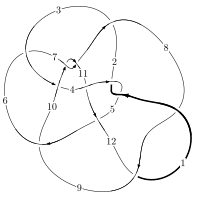
\includegraphics[width=112pt]{../../../GIT/diagram.site/Diagrams/png/2916_12n_0827.png}\\
\ \ \ A knot diagram\footnotemark}&
\allowdisplaybreaks
\textbf{Linearized knot diagam} \\
\cline{2-2}
 &
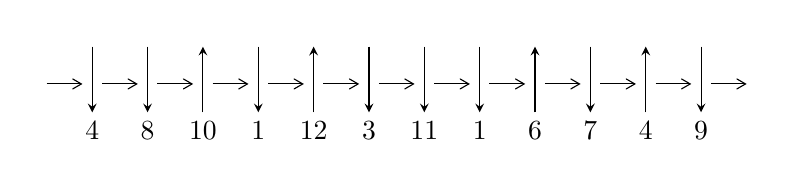
\begin{tikzpicture}[x=20pt, y=17pt]
	% nodes
	\node (C0) at (0, 0) {};
	\node (C1) at (1, 0) {};
	\node (C1U) at (1, +1) {};
	\node (C1D) at (1, -1) {4};

	\node (C2) at (2, 0) {};
	\node (C2U) at (2, +1) {};
	\node (C2D) at (2, -1) {8};

	\node (C3) at (3, 0) {};
	\node (C3U) at (3, +1) {};
	\node (C3D) at (3, -1) {10};

	\node (C4) at (4, 0) {};
	\node (C4U) at (4, +1) {};
	\node (C4D) at (4, -1) {1};

	\node (C5) at (5, 0) {};
	\node (C5U) at (5, +1) {};
	\node (C5D) at (5, -1) {12};

	\node (C6) at (6, 0) {};
	\node (C6U) at (6, +1) {};
	\node (C6D) at (6, -1) {3};

	\node (C7) at (7, 0) {};
	\node (C7U) at (7, +1) {};
	\node (C7D) at (7, -1) {11};

	\node (C8) at (8, 0) {};
	\node (C8U) at (8, +1) {};
	\node (C8D) at (8, -1) {1};

	\node (C9) at (9, 0) {};
	\node (C9U) at (9, +1) {};
	\node (C9D) at (9, -1) {6};

	\node (C10) at (10, 0) {};
	\node (C10U) at (10, +1) {};
	\node (C10D) at (10, -1) {7};

	\node (C11) at (11, 0) {};
	\node (C11U) at (11, +1) {};
	\node (C11D) at (11, -1) {4};

	\node (C12) at (12, 0) {};
	\node (C12U) at (12, +1) {};
	\node (C12D) at (12, -1) {9};
	\node (C13) at (13, 0) {};

	% arrows
	\draw[->,>={angle 60}]
	(C0) edge (C1) (C1) edge (C2) (C2) edge (C3) (C3) edge (C4) (C4) edge (C5) (C5) edge (C6) (C6) edge (C7) (C7) edge (C8) (C8) edge (C9) (C9) edge (C10) (C10) edge (C11) (C11) edge (C12) (C12) edge (C13) ;	\draw[->,>=stealth]
	(C1U) edge (C1D) (C2U) edge (C2D) (C3D) edge (C3U) (C4U) edge (C4D) (C5D) edge (C5U) (C6U) edge (C6D) (C7U) edge (C7D) (C8U) edge (C8D) (C9D) edge (C9U) (C10U) edge (C10D) (C11D) edge (C11U) (C12U) edge (C12D) ;
	\end{tikzpicture} \\
\hhline{~~} \\& 
\textbf{Solving Sequence} \\ \cline{2-2} 
 &
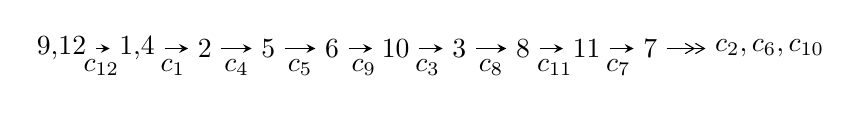
\begin{tikzpicture}[x=23pt, y=7pt]
	% node
	\node (A0) at (-1/8, 0) {9,12};
	\node (A1) at (17/16, 0) {1,4};
	\node (A2) at (17/8, 0) {2};
	\node (A3) at (25/8, 0) {5};
	\node (A4) at (33/8, 0) {6};
	\node (A5) at (41/8, 0) {10};
	\node (A6) at (49/8, 0) {3};
	\node (A7) at (57/8, 0) {8};
	\node (A8) at (65/8, 0) {11};
	\node (A9) at (73/8, 0) {7};
	\node (C1) at (1/2, -1) {$c_{12}$};
	\node (C2) at (13/8, -1) {$c_{1}$};
	\node (C3) at (21/8, -1) {$c_{4}$};
	\node (C4) at (29/8, -1) {$c_{5}$};
	\node (C5) at (37/8, -1) {$c_{9}$};
	\node (C6) at (45/8, -1) {$c_{3}$};
	\node (C7) at (53/8, -1) {$c_{8}$};
	\node (C8) at (61/8, -1) {$c_{11}$};
	\node (C9) at (69/8, -1) {$c_{7}$};
	\node (A10) at (11, 0) {$c_{2},c_{6},c_{10}$};

	% edge
	\draw[->,>=stealth]	
	(A0) edge (A1) (A1) edge (A2) (A2) edge (A3) (A3) edge (A4) (A4) edge (A5) (A5) edge (A6) (A6) edge (A7) (A7) edge (A8) (A8) edge (A9) ;
	\draw[->>,>={angle 60}]	
	(A9) edge (A10);
\end{tikzpicture} \\ 

\end{tabular} \\

\footnotetext{
The image of knot diagram is generated by the software ``\textbf{Draw programme}" developed by Andrew Bartholomew(\url{http://www.layer8.co.uk/maths/draw/index.htm\#Running-draw}), where we modified some parts for our purpose(\url{https://github.com/CATsTAILs/LinksPainter}).
}\phantom \\ \newline 
\centering \textbf{Ideals for irreducible components\footnotemark of $X_{\text{par}}$} 
 
\begin{align*}
I^u_{1}&=\langle 
-1.01535\times10^{193} u^{78}+2.27202\times10^{193} u^{77}+\cdots+1.23813\times10^{195} b+3.31260\times10^{195},\\
\phantom{I^u_{1}}&\phantom{= \langle  }9.77104\times10^{193} u^{78}+4.39315\times10^{194} u^{77}+\cdots+1.23813\times10^{195} a-3.09558\times10^{194},\\
\phantom{I^u_{1}}&\phantom{= \langle  }u^{79}+3 u^{78}+\cdots+200 u+29\rangle \\
I^u_{2}&=\langle 
7428 u^{19}+4394 u^{18}+\cdots+1981 b+11610,\;11189 u^{19}+7253 u^{18}+\cdots+1981 a+3015,\\
\phantom{I^u_{2}}&\phantom{= \langle  }u^{20}+6 u^{18}+\cdots+9 u^2+1\rangle \\
\\
\end{align*}
\raggedright * 2 irreducible components of $\dim_{\mathbb{C}}=0$, with total 99 representations.\\
\footnotetext{All coefficients of polynomials are rational numbers. But the coefficients are sometimes approximated in decimal forms when there is not enough margin.}
\newpage
\renewcommand{\arraystretch}{1}
\centering \section*{I. $I^u_{1}= \langle -1.02\times10^{193} u^{78}+2.27\times10^{193} u^{77}+\cdots+1.24\times10^{195} b+3.31\times10^{195},\;9.77\times10^{193} u^{78}+4.39\times10^{194} u^{77}+\cdots+1.24\times10^{195} a-3.10\times10^{194},\;u^{79}+3 u^{78}+\cdots+200 u+29 \rangle$}
\flushleft \textbf{(i) Arc colorings}\\
\begin{tabular}{m{7pt} m{180pt} m{7pt} m{180pt} }
\flushright $a_{9}=$&$\begin{pmatrix}0\\u\end{pmatrix}$ \\
\flushright $a_{12}=$&$\begin{pmatrix}1\\0\end{pmatrix}$ \\
\flushright $a_{1}=$&$\begin{pmatrix}1\\u^2\end{pmatrix}$ \\
\flushright $a_{4}=$&$\begin{pmatrix}-0.0789177 u^{78}-0.354821 u^{77}+\cdots-1.04936 u+0.250021\\0.00820071 u^{78}-0.0183504 u^{77}+\cdots-10.6030 u-2.67549\end{pmatrix}$ \\
\flushright $a_{2}=$&$\begin{pmatrix}0.316988 u^{78}+0.936300 u^{77}+\cdots+105.357 u+16.3934\\0.238792 u^{78}+0.708289 u^{77}+\cdots+75.5899 u+10.7768\end{pmatrix}$ \\
\flushright $a_{5}=$&$\begin{pmatrix}-0.0251868 u^{78}-0.0941620 u^{77}+\cdots+35.4559 u+6.34948\\-0.0436195 u^{78}-0.194847 u^{77}+\cdots-32.0545 u-5.56001\end{pmatrix}$ \\
\flushright $a_{6}=$&$\begin{pmatrix}-0.0688064 u^{78}-0.289009 u^{77}+\cdots+3.40135 u+0.789464\\-0.0436195 u^{78}-0.194847 u^{77}+\cdots-32.0545 u-5.56001\end{pmatrix}$ \\
\flushright $a_{10}=$&$\begin{pmatrix}0.0169539 u^{78}-0.0560201 u^{77}+\cdots-43.1019 u-7.03695\\-0.0200562 u^{78}-0.0892438 u^{77}+\cdots-24.7956 u-5.58376\end{pmatrix}$ \\
\flushright $a_{3}=$&$\begin{pmatrix}0.270350 u^{78}+0.800990 u^{77}+\cdots+94.9364 u+14.7864\\0.216092 u^{78}+0.639260 u^{77}+\cdots+65.6010 u+9.03626\end{pmatrix}$ \\
\flushright $a_{8}=$&$\begin{pmatrix}u\\u^3+u\end{pmatrix}$ \\
\flushright $a_{11}=$&$\begin{pmatrix}0.104207 u^{78}+0.354515 u^{77}+\cdots+86.3463 u+15.4543\\0.195689 u^{78}+0.613380 u^{77}+\cdots+64.1890 u+9.56182\end{pmatrix}$ \\
\flushright $a_{7}=$&$\begin{pmatrix}-0.0988891 u^{78}-0.365513 u^{77}+\cdots-95.0641 u-17.4083\\-0.199232 u^{78}-0.632045 u^{77}+\cdots-79.9865 u-13.1574\end{pmatrix}$\\&\end{tabular}
\flushleft \textbf{(ii) Obstruction class $= -1$}\\~\\
\flushleft \textbf{(iii) Cusp Shapes $= -0.507381 u^{78}-1.83656 u^{77}+\cdots-237.468 u-36.5233$}\\~\\
\newpage\renewcommand{\arraystretch}{1}
\flushleft \textbf{(iv) u-Polynomials at the component}\newline \\
\begin{tabular}{m{50pt}|m{274pt}}
Crossings & \hspace{64pt}u-Polynomials at each crossing \\
\hline $$\begin{aligned}c_{1},c_{4}\end{aligned}$$&$\begin{aligned}
&u^{79}+11 u^{78}+\cdots+5558 u+2479
\end{aligned}$\\
\hline $$\begin{aligned}c_{2}\end{aligned}$$&$\begin{aligned}
&u^{79}- u^{78}+\cdots-102812253 u+13388083
\end{aligned}$\\
\hline $$\begin{aligned}c_{3}\end{aligned}$$&$\begin{aligned}
&u^{79}+5 u^{76}+\cdots+20 u+1
\end{aligned}$\\
\hline $$\begin{aligned}c_{5}\end{aligned}$$&$\begin{aligned}
&u^{79}+5 u^{78}+\cdots+13423495 u+1556833
\end{aligned}$\\
\hline $$\begin{aligned}c_{6}\end{aligned}$$&$\begin{aligned}
&u^{79}+7 u^{78}+\cdots+68 u-7
\end{aligned}$\\
\hline $$\begin{aligned}c_{7},c_{10}\end{aligned}$$&$\begin{aligned}
&u^{79}+u^{78}+\cdots+77 u+19
\end{aligned}$\\
\hline $$\begin{aligned}c_{8},c_{12}\end{aligned}$$&$\begin{aligned}
&u^{79}+3 u^{78}+\cdots+200 u+29
\end{aligned}$\\
\hline $$\begin{aligned}c_{9}\end{aligned}$$&$\begin{aligned}
&u^{79}- u^{78}+\cdots-8553 u+4021
\end{aligned}$\\
\hline $$\begin{aligned}c_{11}\end{aligned}$$&$\begin{aligned}
&u^{79}-3 u^{78}+\cdots+7160839 u+2429981
\end{aligned}$\\
\hline
\end{tabular}\\~\\
\newpage\renewcommand{\arraystretch}{1}
\flushleft \textbf{(v) Riley Polynomials at the component}\newline \\
\begin{tabular}{m{50pt}|m{274pt}}
Crossings & \hspace{64pt}Riley Polynomials at each crossing \\
\hline $$\begin{aligned}c_{1},c_{4}\end{aligned}$$&$\begin{aligned}
&y^{79}-77 y^{78}+\cdots+415458634 y-6145441
\end{aligned}$\\
\hline $$\begin{aligned}c_{2}\end{aligned}$$&$\begin{aligned}
&y^{79}-57 y^{78}+\cdots+3295984311821017 y-179240766414889
\end{aligned}$\\
\hline $$\begin{aligned}c_{3}\end{aligned}$$&$\begin{aligned}
&y^{79}+86 y^{77}+\cdots-12 y-1
\end{aligned}$\\
\hline $$\begin{aligned}c_{5}\end{aligned}$$&$\begin{aligned}
&y^{79}+39 y^{78}+\cdots-73169724732107 y-2423728989889
\end{aligned}$\\
\hline $$\begin{aligned}c_{6}\end{aligned}$$&$\begin{aligned}
&y^{79}- y^{78}+\cdots+1306 y-49
\end{aligned}$\\
\hline $$\begin{aligned}c_{7},c_{10}\end{aligned}$$&$\begin{aligned}
&y^{79}-61 y^{78}+\cdots-21393 y-361
\end{aligned}$\\
\hline $$\begin{aligned}c_{8},c_{12}\end{aligned}$$&$\begin{aligned}
&y^{79}+23 y^{78}+\cdots-15912 y-841
\end{aligned}$\\
\hline $$\begin{aligned}c_{9}\end{aligned}$$&$\begin{aligned}
&y^{79}-45 y^{78}+\cdots+347635311 y-16168441
\end{aligned}$\\
\hline $$\begin{aligned}c_{11}\end{aligned}$$&$\begin{aligned}
&y^{79}+43 y^{78}+\cdots-76836824810403 y-5904807660361
\end{aligned}$\\
\hline
\end{tabular}\\~\\
\newpage\flushleft \textbf{(vi) Complex Volumes and Cusp Shapes}
$$\begin{array}{c|c|c}  
\text{Solutions to }I^u_{1}& \I (\text{vol} + \sqrt{-1}CS) & \text{Cusp shape}\\
 \hline 
\begin{aligned}
u &= -0.365028 + 0.921649 I \\
a &= \phantom{-}0.485538 - 0.442665 I \\
b &= -1.012030 - 0.390280 I\end{aligned}
 & \phantom{-}0.81357 + 3.15646 I & \phantom{-0.000000 } 0 \\ \hline\begin{aligned}
u &= -0.365028 - 0.921649 I \\
a &= \phantom{-}0.485538 + 0.442665 I \\
b &= -1.012030 + 0.390280 I\end{aligned}
 & \phantom{-}0.81357 - 3.15646 I & \phantom{-0.000000 } 0 \\ \hline\begin{aligned}
u &= -0.048716 + 0.988429 I \\
a &= \phantom{-}1.05917 + 2.15503 I \\
b &= -0.547677 - 0.774768 I\end{aligned}
 & \phantom{-}2.98173 - 4.48398 I & \phantom{-0.000000 } 0 \\ \hline\begin{aligned}
u &= -0.048716 - 0.988429 I \\
a &= \phantom{-}1.05917 - 2.15503 I \\
b &= -0.547677 + 0.774768 I\end{aligned}
 & \phantom{-}2.98173 + 4.48398 I & \phantom{-0.000000 } 0 \\ \hline\begin{aligned}
u &= -0.550088 + 0.820510 I \\
a &= -1.232910 + 0.211959 I \\
b &= \phantom{-}0.901767 + 0.418938 I\end{aligned}
 & \phantom{-}0.35934 + 8.67454 I & \phantom{-0.000000 } 0 \\ \hline\begin{aligned}
u &= -0.550088 - 0.820510 I \\
a &= -1.232910 - 0.211959 I \\
b &= \phantom{-}0.901767 - 0.418938 I\end{aligned}
 & \phantom{-}0.35934 - 8.67454 I & \phantom{-0.000000 } 0 \\ \hline\begin{aligned}
u &= \phantom{-}0.769309 + 0.614688 I \\
a &= \phantom{-}0.106252 + 1.084980 I \\
b &= \phantom{-}0.466533 + 0.733029 I\end{aligned}
 & -3.16503 - 1.16137 I & \phantom{-0.000000 } 0 \\ \hline\begin{aligned}
u &= \phantom{-}0.769309 - 0.614688 I \\
a &= \phantom{-}0.106252 - 1.084980 I \\
b &= \phantom{-}0.466533 - 0.733029 I\end{aligned}
 & -3.16503 + 1.16137 I & \phantom{-0.000000 } 0 \\ \hline\begin{aligned}
u &= -0.198767 + 0.920559 I \\
a &= \phantom{-}0.232424 - 0.455553 I \\
b &= -1.054030 - 0.576556 I\end{aligned}
 & \phantom{-}0.56704 + 3.08659 I & \phantom{-0.000000 } 0 \\ \hline\begin{aligned}
u &= -0.198767 - 0.920559 I \\
a &= \phantom{-}0.232424 + 0.455553 I \\
b &= -1.054030 + 0.576556 I\end{aligned}
 & \phantom{-}0.56704 - 3.08659 I & \phantom{-0.000000 } 0\\
 \hline 
 \end{array}$$\newpage$$\begin{array}{c|c|c}  
\text{Solutions to }I^u_{1}& \I (\text{vol} + \sqrt{-1}CS) & \text{Cusp shape}\\
 \hline 
\begin{aligned}
u &= -0.697347 + 0.814961 I \\
a &= \phantom{-}0.27962 - 2.05303 I \\
b &= -0.633965 - 0.761739 I\end{aligned}
 & -6.29169 + 2.64828 I & \phantom{-0.000000 } 0 \\ \hline\begin{aligned}
u &= -0.697347 - 0.814961 I \\
a &= \phantom{-}0.27962 + 2.05303 I \\
b &= -0.633965 + 0.761739 I\end{aligned}
 & -6.29169 - 2.64828 I & \phantom{-0.000000 } 0 \\ \hline\begin{aligned}
u &= -1.048100 + 0.403578 I \\
a &= \phantom{-}0.808674 - 0.404445 I \\
b &= \phantom{-}2.32569 - 1.11746 I\end{aligned}
 & -7.15287 + 0.34372 I & \phantom{-0.000000 } 0 \\ \hline\begin{aligned}
u &= -1.048100 - 0.403578 I \\
a &= \phantom{-}0.808674 + 0.404445 I \\
b &= \phantom{-}2.32569 + 1.11746 I\end{aligned}
 & -7.15287 - 0.34372 I & \phantom{-0.000000 } 0 \\ \hline\begin{aligned}
u &= \phantom{-}0.383423 + 0.764569 I \\
a &= \phantom{-}0.255771 + 0.433790 I \\
b &= -1.276420 - 0.222595 I\end{aligned}
 & \phantom{-}4.18971 + 0.51454 I & \phantom{-}2.17923 + 0. I\phantom{ +0.000000I} \\ \hline\begin{aligned}
u &= \phantom{-}0.383423 - 0.764569 I \\
a &= \phantom{-}0.255771 - 0.433790 I \\
b &= -1.276420 + 0.222595 I\end{aligned}
 & \phantom{-}4.18971 - 0.51454 I & \phantom{-}2.17923 + 0. I\phantom{ +0.000000I} \\ \hline\begin{aligned}
u &= -0.620381 + 0.965544 I \\
a &= \phantom{-}1.12040 - 1.00106 I \\
b &= \phantom{-}0.280816 - 0.558368 I\end{aligned}
 & -5.81347 + 2.47228 I & \phantom{-0.000000 } 0 \\ \hline\begin{aligned}
u &= -0.620381 - 0.965544 I \\
a &= \phantom{-}1.12040 + 1.00106 I \\
b &= \phantom{-}0.280816 + 0.558368 I\end{aligned}
 & -5.81347 - 2.47228 I & \phantom{-0.000000 } 0 \\ \hline\begin{aligned}
u &= -0.946796 + 0.663690 I \\
a &= \phantom{-}0.148069 + 1.213100 I \\
b &= \phantom{-}0.525674 + 0.797143 I\end{aligned}
 & -4.51817 + 2.00997 I & \phantom{-0.000000 } 0 \\ \hline\begin{aligned}
u &= -0.946796 - 0.663690 I \\
a &= \phantom{-}0.148069 - 1.213100 I \\
b &= \phantom{-}0.525674 - 0.797143 I\end{aligned}
 & -4.51817 - 2.00997 I & \phantom{-0.000000 } 0\\
 \hline 
 \end{array}$$\newpage$$\begin{array}{c|c|c}  
\text{Solutions to }I^u_{1}& \I (\text{vol} + \sqrt{-1}CS) & \text{Cusp shape}\\
 \hline 
\begin{aligned}
u &= -0.478436 + 0.694599 I \\
a &= \phantom{-}0.244214 - 0.318915 I \\
b &= -1.098680 + 0.795145 I\end{aligned}
 & \phantom{-}0.01895 - 4.62268 I & -4.00000 + 2.42967 I \\ \hline\begin{aligned}
u &= -0.478436 - 0.694599 I \\
a &= \phantom{-}0.244214 + 0.318915 I \\
b &= -1.098680 - 0.795145 I\end{aligned}
 & \phantom{-}0.01895 + 4.62268 I & -4.00000 - 2.42967 I \\ \hline\begin{aligned}
u &= \phantom{-}0.816484 + 0.827857 I \\
a &= \phantom{-}1.04084 + 1.10388 I \\
b &= \phantom{-}0.165023 + 1.149580 I\end{aligned}
 & -6.08738 + 0.90469 I & \phantom{-0.000000 } 0 \\ \hline\begin{aligned}
u &= \phantom{-}0.816484 - 0.827857 I \\
a &= \phantom{-}1.04084 - 1.10388 I \\
b &= \phantom{-}0.165023 - 1.149580 I\end{aligned}
 & -6.08738 - 0.90469 I & \phantom{-0.000000 } 0 \\ \hline\begin{aligned}
u &= \phantom{-}0.226560 + 0.796466 I \\
a &= \phantom{-}1.74735 - 0.47514 I \\
b &= -0.512841 + 0.571552 I\end{aligned}
 & -1.96522 + 0.47763 I & -4.53788 + 0.92547 I \\ \hline\begin{aligned}
u &= \phantom{-}0.226560 - 0.796466 I \\
a &= \phantom{-}1.74735 + 0.47514 I \\
b &= -0.512841 - 0.571552 I\end{aligned}
 & -1.96522 - 0.47763 I & -4.53788 - 0.92547 I \\ \hline\begin{aligned}
u &= \phantom{-}0.475780 + 0.661767 I \\
a &= -0.91811 - 1.22985 I \\
b &= \phantom{-}1.185730 - 0.177054 I\end{aligned}
 & \phantom{-}3.73228 - 3.86132 I & -1.05530 + 7.68432 I \\ \hline\begin{aligned}
u &= \phantom{-}0.475780 - 0.661767 I \\
a &= -0.91811 + 1.22985 I \\
b &= \phantom{-}1.185730 + 0.177054 I\end{aligned}
 & \phantom{-}3.73228 + 3.86132 I & -1.05530 - 7.68432 I \\ \hline\begin{aligned}
u &= \phantom{-}0.769284 + 0.247205 I \\
a &= \phantom{-}0.088417 + 0.987187 I \\
b &= \phantom{-}0.11862 + 1.57494 I\end{aligned}
 & -4.09349 - 3.57659 I & -10.32261 + 5.90091 I \\ \hline\begin{aligned}
u &= \phantom{-}0.769284 - 0.247205 I \\
a &= \phantom{-}0.088417 - 0.987187 I \\
b &= \phantom{-}0.11862 - 1.57494 I\end{aligned}
 & -4.09349 + 3.57659 I & -10.32261 - 5.90091 I\\
 \hline 
 \end{array}$$\newpage$$\begin{array}{c|c|c}  
\text{Solutions to }I^u_{1}& \I (\text{vol} + \sqrt{-1}CS) & \text{Cusp shape}\\
 \hline 
\begin{aligned}
u &= \phantom{-}1.029470 + 0.653797 I \\
a &= -0.406332 - 0.758563 I \\
b &= -0.583979 - 1.033370 I\end{aligned}
 & -1.60411 + 4.69680 I & \phantom{-0.000000 } 0 \\ \hline\begin{aligned}
u &= \phantom{-}1.029470 - 0.653797 I \\
a &= -0.406332 + 0.758563 I \\
b &= -0.583979 + 1.033370 I\end{aligned}
 & -1.60411 - 4.69680 I & \phantom{-0.000000 } 0 \\ \hline\begin{aligned}
u &= \phantom{-}0.787331 + 0.948348 I \\
a &= \phantom{-}0.48663 + 1.51737 I \\
b &= -0.436525 + 1.341180 I\end{aligned}
 & -5.72001 - 6.91767 I & \phantom{-0.000000 } 0 \\ \hline\begin{aligned}
u &= \phantom{-}0.787331 - 0.948348 I \\
a &= \phantom{-}0.48663 - 1.51737 I \\
b &= -0.436525 - 1.341180 I\end{aligned}
 & -5.72001 + 6.91767 I & \phantom{-0.000000 } 0 \\ \hline\begin{aligned}
u &= \phantom{-}0.277595 + 0.709657 I \\
a &= -0.42118 + 1.83706 I \\
b &= -0.866044 + 0.759028 I\end{aligned}
 & \phantom{-}4.81405 - 3.49144 I & \phantom{-}1.70169 + 10.64917 I \\ \hline\begin{aligned}
u &= \phantom{-}0.277595 - 0.709657 I \\
a &= -0.42118 - 1.83706 I \\
b &= -0.866044 - 0.759028 I\end{aligned}
 & \phantom{-}4.81405 + 3.49144 I & \phantom{-}1.70169 - 10.64917 I \\ \hline\begin{aligned}
u &= -0.878531 + 0.877785 I \\
a &= \phantom{-}0.635036 - 1.147060 I \\
b &= -0.508946 - 1.300500 I\end{aligned}
 & -2.18564 + 1.23495 I & \phantom{-0.000000 } 0 \\ \hline\begin{aligned}
u &= -0.878531 - 0.877785 I \\
a &= \phantom{-}0.635036 + 1.147060 I \\
b &= -0.508946 + 1.300500 I\end{aligned}
 & -2.18564 - 1.23495 I & \phantom{-0.000000 } 0 \\ \hline\begin{aligned}
u &= \phantom{-}0.192145 + 0.711068 I \\
a &= \phantom{-}0.73682 - 2.59438 I \\
b &= \phantom{-}0.499627 + 0.054033 I\end{aligned}
 & \phantom{-}4.89202 + 1.47198 I & \phantom{-}0.48436 + 2.56488 I \\ \hline\begin{aligned}
u &= \phantom{-}0.192145 - 0.711068 I \\
a &= \phantom{-}0.73682 + 2.59438 I \\
b &= \phantom{-}0.499627 - 0.054033 I\end{aligned}
 & \phantom{-}4.89202 - 1.47198 I & \phantom{-}0.48436 - 2.56488 I\\
 \hline 
 \end{array}$$\newpage$$\begin{array}{c|c|c}  
\text{Solutions to }I^u_{1}& \I (\text{vol} + \sqrt{-1}CS) & \text{Cusp shape}\\
 \hline 
\begin{aligned}
u &= -0.857032 + 0.937871 I \\
a &= \phantom{-}0.652099 - 0.879166 I \\
b &= \phantom{-}0.16783 - 1.46825 I\end{aligned}
 & -2.00049 + 5.18597 I & \phantom{-0.000000 } 0 \\ \hline\begin{aligned}
u &= -0.857032 - 0.937871 I \\
a &= \phantom{-}0.652099 + 0.879166 I \\
b &= \phantom{-}0.16783 + 1.46825 I\end{aligned}
 & -2.00049 - 5.18597 I & \phantom{-0.000000 } 0 \\ \hline\begin{aligned}
u &= -1.099410 + 0.697283 I \\
a &= -0.819118 + 0.794230 I \\
b &= -1.07548 + 1.77879 I\end{aligned}
 & -6.68531 - 9.94778 I & \phantom{-0.000000 } 0 \\ \hline\begin{aligned}
u &= -1.099410 - 0.697283 I \\
a &= -0.819118 - 0.794230 I \\
b &= -1.07548 - 1.77879 I\end{aligned}
 & -6.68531 + 9.94778 I & \phantom{-0.000000 } 0 \\ \hline\begin{aligned}
u &= \phantom{-}0.963490 + 0.926074 I \\
a &= -0.855656 - 0.607154 I \\
b &= -0.67372 - 1.46186 I\end{aligned}
 & -9.63489 + 3.13405 I & \phantom{-0.000000 } 0 \\ \hline\begin{aligned}
u &= \phantom{-}0.963490 - 0.926074 I \\
a &= -0.855656 + 0.607154 I \\
b &= -0.67372 + 1.46186 I\end{aligned}
 & -9.63489 - 3.13405 I & \phantom{-0.000000 } 0 \\ \hline\begin{aligned}
u &= \phantom{-}0.923648 + 0.974917 I \\
a &= -0.46630 - 1.42944 I \\
b &= \phantom{-}1.03334 - 1.39055 I\end{aligned}
 & -9.46238 - 10.03940 I & \phantom{-0.000000 } 0 \\ \hline\begin{aligned}
u &= \phantom{-}0.923648 - 0.974917 I \\
a &= -0.46630 + 1.42944 I \\
b &= \phantom{-}1.03334 + 1.39055 I\end{aligned}
 & -9.46238 + 10.03940 I & \phantom{-0.000000 } 0 \\ \hline\begin{aligned}
u &= -0.329773 + 1.305820 I \\
a &= -0.270422 - 0.326511 I \\
b &= -0.261756 + 0.423075 I\end{aligned}
 & \phantom{-}1.86473 + 3.78804 I & \phantom{-0.000000 } 0 \\ \hline\begin{aligned}
u &= -0.329773 - 1.305820 I \\
a &= -0.270422 + 0.326511 I \\
b &= -0.261756 - 0.423075 I\end{aligned}
 & \phantom{-}1.86473 - 3.78804 I & \phantom{-0.000000 } 0\\
 \hline 
 \end{array}$$\newpage$$\begin{array}{c|c|c}  
\text{Solutions to }I^u_{1}& \I (\text{vol} + \sqrt{-1}CS) & \text{Cusp shape}\\
 \hline 
\begin{aligned}
u &= \phantom{-}0.701774 + 1.150670 I \\
a &= \phantom{-}0.86461 + 1.13965 I \\
b &= -0.950853 + 0.756054 I\end{aligned}
 & -1.45140 - 4.50648 I & \phantom{-0.000000 } 0 \\ \hline\begin{aligned}
u &= \phantom{-}0.701774 - 1.150670 I \\
a &= \phantom{-}0.86461 - 1.13965 I \\
b &= -0.950853 - 0.756054 I\end{aligned}
 & -1.45140 + 4.50648 I & \phantom{-0.000000 } 0 \\ \hline\begin{aligned}
u &= -0.972873 + 0.937650 I \\
a &= -0.295198 + 0.885473 I \\
b &= \phantom{-}0.260392 + 0.884421 I\end{aligned}
 & -4.28133 + 3.53574 I & \phantom{-0.000000 } 0 \\ \hline\begin{aligned}
u &= -0.972873 - 0.937650 I \\
a &= -0.295198 - 0.885473 I \\
b &= \phantom{-}0.260392 - 0.884421 I\end{aligned}
 & -4.28133 - 3.53574 I & \phantom{-0.000000 } 0 \\ \hline\begin{aligned}
u &= -0.821478 + 1.130920 I \\
a &= -0.548820 + 0.572288 I \\
b &= -0.037613 + 0.738202 I\end{aligned}
 & -3.08625 + 4.54824 I & \phantom{-0.000000 } 0 \\ \hline\begin{aligned}
u &= -0.821478 - 1.130920 I \\
a &= -0.548820 - 0.572288 I \\
b &= -0.037613 - 0.738202 I\end{aligned}
 & -3.08625 - 4.54824 I & \phantom{-0.000000 } 0 \\ \hline\begin{aligned}
u &= -0.599388\phantom{ +0.000000I} \\
a &= \phantom{-}1.13836\phantom{ +0.000000I} \\
b &= \phantom{-}0.628716\phantom{ +0.000000I}\end{aligned}
 & -1.88001\phantom{ +0.000000I} & -6.12910\phantom{ +0.000000I} \\ \hline\begin{aligned}
u &= \phantom{-}0.821578 + 1.137080 I \\
a &= -0.605483 - 1.147130 I \\
b &= \phantom{-}0.885700 - 0.997087 I\end{aligned}
 & -0.11191 - 11.43530 I & \phantom{-0.000000 } 0 \\ \hline\begin{aligned}
u &= \phantom{-}0.821578 - 1.137080 I \\
a &= -0.605483 + 1.147130 I \\
b &= \phantom{-}0.885700 + 0.997087 I\end{aligned}
 & -0.11191 + 11.43530 I & \phantom{-0.000000 } 0 \\ \hline\begin{aligned}
u &= \phantom{-}1.080490 + 0.909752 I \\
a &= \phantom{-}0.69148 + 1.34893 I \\
b &= -1.01470 + 2.67163 I\end{aligned}
 & -5.52397 - 3.79706 I & \phantom{-0.000000 } 0\\
 \hline 
 \end{array}$$\newpage$$\begin{array}{c|c|c}  
\text{Solutions to }I^u_{1}& \I (\text{vol} + \sqrt{-1}CS) & \text{Cusp shape}\\
 \hline 
\begin{aligned}
u &= \phantom{-}1.080490 - 0.909752 I \\
a &= \phantom{-}0.69148 - 1.34893 I \\
b &= -1.01470 - 2.67163 I\end{aligned}
 & -5.52397 + 3.79706 I & \phantom{-0.000000 } 0 \\ \hline\begin{aligned}
u &= \phantom{-}0.054786 + 1.411470 I \\
a &= -0.326149 - 0.219838 I \\
b &= \phantom{-}0.324393 + 0.617013 I\end{aligned}
 & \phantom{-}6.16628 + 1.89006 I & \phantom{-0.000000 } 0 \\ \hline\begin{aligned}
u &= \phantom{-}0.054786 - 1.411470 I \\
a &= -0.326149 + 0.219838 I \\
b &= \phantom{-}0.324393 - 0.617013 I\end{aligned}
 & \phantom{-}6.16628 - 1.89006 I & \phantom{-0.000000 } 0 \\ \hline\begin{aligned}
u &= -0.312943 + 0.477853 I \\
a &= -1.14468 - 2.44162 I \\
b &= -0.63512 - 1.78649 I\end{aligned}
 & \phantom{-}0.79605 + 6.21294 I & -6.33131 - 10.12425 I \\ \hline\begin{aligned}
u &= -0.312943 - 0.477853 I \\
a &= -1.14468 + 2.44162 I \\
b &= -0.63512 + 1.78649 I\end{aligned}
 & \phantom{-}0.79605 - 6.21294 I & -6.33131 + 10.12425 I \\ \hline\begin{aligned}
u &= -0.85067 + 1.14814 I \\
a &= -0.83436 + 1.42013 I \\
b &= \phantom{-}1.35640 + 1.56095 I\end{aligned}
 & -5.2404 + 16.9790 I & \phantom{-0.000000 } 0 \\ \hline\begin{aligned}
u &= -0.85067 - 1.14814 I \\
a &= -0.83436 - 1.42013 I \\
b &= \phantom{-}1.35640 - 1.56095 I\end{aligned}
 & -5.2404 - 16.9790 I & \phantom{-0.000000 } 0 \\ \hline\begin{aligned}
u &= \phantom{-}1.09269 + 0.93791 I \\
a &= \phantom{-}1.307310 + 0.521345 I \\
b &= \phantom{-}1.29376 + 3.00284 I\end{aligned}
 & -5.47068 - 3.91698 I & \phantom{-0.000000 } 0 \\ \hline\begin{aligned}
u &= \phantom{-}1.09269 - 0.93791 I \\
a &= \phantom{-}1.307310 - 0.521345 I \\
b &= \phantom{-}1.29376 - 3.00284 I\end{aligned}
 & -5.47068 + 3.91698 I & \phantom{-0.000000 } 0 \\ \hline\begin{aligned}
u &= -0.487872 + 0.175765 I \\
a &= \phantom{-}1.76241 + 1.10617 I \\
b &= \phantom{-}1.137630 + 0.211015 I\end{aligned}
 & -1.82613 + 0.02881 I & -6.76412 + 0.34713 I\\
 \hline 
 \end{array}$$\newpage$$\begin{array}{c|c|c}  
\text{Solutions to }I^u_{1}& \I (\text{vol} + \sqrt{-1}CS) & \text{Cusp shape}\\
 \hline 
\begin{aligned}
u &= -0.487872 - 0.175765 I \\
a &= \phantom{-}1.76241 - 1.10617 I \\
b &= \phantom{-}1.137630 - 0.211015 I\end{aligned}
 & -1.82613 - 0.02881 I & -6.76412 - 0.34713 I \\ \hline\begin{aligned}
u &= -0.370186 + 0.350900 I \\
a &= \phantom{-}0.573493 - 0.938784 I \\
b &= -0.096093 - 0.493512 I\end{aligned}
 & -0.270088 + 1.031330 I & -4.41640 - 6.52686 I \\ \hline\begin{aligned}
u &= -0.370186 - 0.350900 I \\
a &= \phantom{-}0.573493 + 0.938784 I \\
b &= -0.096093 + 0.493512 I\end{aligned}
 & -0.270088 - 1.031330 I & -4.41640 + 6.52686 I \\ \hline\begin{aligned}
u &= \phantom{-}0.13902 + 1.49464 I \\
a &= -0.298338 + 0.663603 I \\
b &= \phantom{-}0.24627 - 1.50057 I\end{aligned}
 & \phantom{-}2.55162 - 7.07486 I & \phantom{-0.000000 } 0 \\ \hline\begin{aligned}
u &= \phantom{-}0.13902 - 1.49464 I \\
a &= -0.298338 - 0.663603 I \\
b &= \phantom{-}0.24627 + 1.50057 I\end{aligned}
 & \phantom{-}2.55162 + 7.07486 I & \phantom{-0.000000 } 0 \\ \hline\begin{aligned}
u &= \phantom{-}0.124655 + 0.464854 I \\
a &= -3.09093 + 1.14602 I \\
b &= \phantom{-}0.823635 - 0.304659 I\end{aligned}
 & -1.18700 - 2.75544 I & -3.0625 + 14.8135 I \\ \hline\begin{aligned}
u &= \phantom{-}0.124655 - 0.464854 I \\
a &= -3.09093 - 1.14602 I \\
b &= \phantom{-}0.823635 + 0.304659 I\end{aligned}
 & -1.18700 + 2.75544 I & -3.0625 - 14.8135 I \\ \hline\begin{aligned}
u &= -0.89541 + 1.30049 I \\
a &= \phantom{-}1.05199 - 1.41768 I \\
b &= -2.53671 - 1.97919 I\end{aligned}
 & -4.46745 + 6.91864 I & \phantom{-0.000000 } 0 \\ \hline\begin{aligned}
u &= -0.89541 - 1.30049 I \\
a &= \phantom{-}1.05199 + 1.41768 I \\
b &= -2.53671 + 1.97919 I\end{aligned}
 & -4.46745 - 6.91864 I & \phantom{-0.000000 } 0\\
 \hline 
 \end{array}$$\newpage\newpage\renewcommand{\arraystretch}{1}
\centering \section*{II. $I^u_{2}= \langle 7428 u^{19}+4394 u^{18}+\cdots+1981 b+11610,\;11189 u^{19}+7253 u^{18}+\cdots+1981 a+3015,\;u^{20}+6 u^{18}+\cdots+9 u^2+1 \rangle$}
\flushleft \textbf{(i) Arc colorings}\\
\begin{tabular}{m{7pt} m{180pt} m{7pt} m{180pt} }
\flushright $a_{9}=$&$\begin{pmatrix}0\\u\end{pmatrix}$ \\
\flushright $a_{12}=$&$\begin{pmatrix}1\\0\end{pmatrix}$ \\
\flushright $a_{1}=$&$\begin{pmatrix}1\\u^2\end{pmatrix}$ \\
\flushright $a_{4}=$&$\begin{pmatrix}-5.64816 u^{19}-3.66128 u^{18}+\cdots-15.9192 u-1.52196\\-3.74962 u^{19}-2.21807 u^{18}+\cdots-8.27108 u-5.86068\end{pmatrix}$ \\
\flushright $a_{2}=$&$\begin{pmatrix}4.50278 u^{19}-5.59919 u^{18}+\cdots+17.0121 u-13.9783\\11.9086 u^{19}+1.62797 u^{18}+\cdots+28.4195 u+1.37658\end{pmatrix}$ \\
\flushright $a_{5}=$&$\begin{pmatrix}u^{18}+6 u^{16}+\cdots-2 u+8\\-5.64816 u^{19}-4.66128 u^{18}+\cdots-13.9192 u-10.5220\end{pmatrix}$ \\
\flushright $a_{6}=$&$\begin{pmatrix}-5.64816 u^{19}-3.66128 u^{18}+\cdots-15.9192 u-2.52196\\-5.64816 u^{19}-4.66128 u^{18}+\cdots-13.9192 u-10.5220\end{pmatrix}$ \\
\flushright $a_{10}=$&$\begin{pmatrix}-1.02373 u^{19}-0.334175 u^{18}+\cdots+0.987380 u-1.73094\\-2.16305 u^{19}-4.08380 u^{18}+\cdots-10.2569 u-12.0020\end{pmatrix}$ \\
\flushright $a_{3}=$&$\begin{pmatrix}8.25240 u^{19}-3.38112 u^{18}+\cdots+25.2832 u-9.11762\\14.0490 u^{19}+2.79606 u^{18}+\cdots+32.9409 u+4.01918\end{pmatrix}$ \\
\flushright $a_{8}=$&$\begin{pmatrix}u\\u^3+u\end{pmatrix}$ \\
\flushright $a_{11}=$&$\begin{pmatrix}7.38718 u^{19}-2.01464 u^{18}+\cdots+22.7804 u-10.5184\\9.34074 u^{19}+1.73549 u^{18}+\cdots+21.0323 u+3.39122\end{pmatrix}$ \\
\flushright $a_{7}=$&$\begin{pmatrix}9.38213 u^{19}-0.107017 u^{18}+\cdots+21.3948 u+2.62393\\7.13074 u^{19}+3.69258 u^{18}+\cdots+19.3887 u+6.11307\end{pmatrix}$\\&\end{tabular}
\flushleft \textbf{(ii) Obstruction class $= 1$}\\~\\
\flushleft \textbf{(iii) Cusp Shapes $= -\frac{28246}{1981} u^{19}-\frac{10162}{1981} u^{18}+\cdots-\frac{120734}{1981} u-\frac{22012}{1981}$}\\~\\
\newpage\renewcommand{\arraystretch}{1}
\flushleft \textbf{(iv) u-Polynomials at the component}\newline \\
\begin{tabular}{m{50pt}|m{274pt}}
Crossings & \hspace{64pt}u-Polynomials at each crossing \\
\hline $$\begin{aligned}c_{1}\end{aligned}$$&$\begin{aligned}
&u^{20}-12 u^{19}+\cdots-74 u+11
\end{aligned}$\\
\hline $$\begin{aligned}c_{2}\end{aligned}$$&$\begin{aligned}
&u^{20}-8 u^{18}+\cdots+117 u+59
\end{aligned}$\\
\hline $$\begin{aligned}c_{3}\end{aligned}$$&$\begin{aligned}
&u^{20}+u^{19}+\cdots-2 u+1
\end{aligned}$\\
\hline $$\begin{aligned}c_{4}\end{aligned}$$&$\begin{aligned}
&u^{20}+12 u^{19}+\cdots+74 u+11
\end{aligned}$\\
\hline $$\begin{aligned}c_{5}\end{aligned}$$&$\begin{aligned}
&u^{20}+4 u^{19}+\cdots+293 u+101
\end{aligned}$\\
\hline $$\begin{aligned}c_{6}\end{aligned}$$&$\begin{aligned}
&u^{20}+2 u^{18}+\cdots+4 u+1
\end{aligned}$\\
\hline $$\begin{aligned}c_{7}\end{aligned}$$&$\begin{aligned}
&u^{20}-8 u^{18}+\cdots+5 u+7
\end{aligned}$\\
\hline $$\begin{aligned}c_{8}\end{aligned}$$&$\begin{aligned}
&u^{20}+6 u^{18}+\cdots+9 u^2+1
\end{aligned}$\\
\hline $$\begin{aligned}c_{9}\end{aligned}$$&$\begin{aligned}
&u^{20}-8 u^{18}+\cdots-11 u+7
\end{aligned}$\\
\hline $$\begin{aligned}c_{10}\end{aligned}$$&$\begin{aligned}
&u^{20}-8 u^{18}+\cdots-5 u+7
\end{aligned}$\\
\hline $$\begin{aligned}c_{11}\end{aligned}$$&$\begin{aligned}
&u^{20}+4 u^{19}+\cdots-11 u+7
\end{aligned}$\\
\hline $$\begin{aligned}c_{12}\end{aligned}$$&$\begin{aligned}
&u^{20}+6 u^{18}+\cdots+9 u^2+1
\end{aligned}$\\
\hline
\end{tabular}\\~\\
\newpage\renewcommand{\arraystretch}{1}
\flushleft \textbf{(v) Riley Polynomials at the component}\newline \\
\begin{tabular}{m{50pt}|m{274pt}}
Crossings & \hspace{64pt}Riley Polynomials at each crossing \\
\hline $$\begin{aligned}c_{1},c_{4}\end{aligned}$$&$\begin{aligned}
&y^{20}-4 y^{19}+\cdots+112 y+121
\end{aligned}$\\
\hline $$\begin{aligned}c_{2}\end{aligned}$$&$\begin{aligned}
&y^{20}-16 y^{19}+\cdots-20887 y+3481
\end{aligned}$\\
\hline $$\begin{aligned}c_{3}\end{aligned}$$&$\begin{aligned}
&y^{20}-3 y^{19}+\cdots-6 y+1
\end{aligned}$\\
\hline $$\begin{aligned}c_{5}\end{aligned}$$&$\begin{aligned}
&y^{20}+12 y^{19}+\cdots+51713 y+10201
\end{aligned}$\\
\hline $$\begin{aligned}c_{6}\end{aligned}$$&$\begin{aligned}
&y^{20}+4 y^{19}+\cdots+8 y+1
\end{aligned}$\\
\hline $$\begin{aligned}c_{7},c_{10}\end{aligned}$$&$\begin{aligned}
&y^{20}-16 y^{19}+\cdots-53 y+49
\end{aligned}$\\
\hline $$\begin{aligned}c_{8},c_{12}\end{aligned}$$&$\begin{aligned}
&y^{20}+12 y^{19}+\cdots+18 y+1
\end{aligned}$\\
\hline $$\begin{aligned}c_{9}\end{aligned}$$&$\begin{aligned}
&y^{20}-16 y^{19}+\cdots-513 y+49
\end{aligned}$\\
\hline $$\begin{aligned}c_{11}\end{aligned}$$&$\begin{aligned}
&y^{20}+12 y^{19}+\cdots-51 y+49
\end{aligned}$\\
\hline
\end{tabular}\\~\\
\newpage\flushleft \textbf{(vi) Complex Volumes and Cusp Shapes}
$$\begin{array}{c|c|c}  
\text{Solutions to }I^u_{2}& \I (\text{vol} + \sqrt{-1}CS) & \text{Cusp shape}\\
 \hline 
\begin{aligned}
u &= \phantom{-}0.768071 + 0.596737 I \\
a &= \phantom{-}0.604655 + 1.101940 I \\
b &= \phantom{-}0.997208 + 0.889634 I\end{aligned}
 & -6.10903 - 0.54639 I & -6.35226 + 0.28610 I \\ \hline\begin{aligned}
u &= \phantom{-}0.768071 - 0.596737 I \\
a &= \phantom{-}0.604655 - 1.101940 I \\
b &= \phantom{-}0.997208 - 0.889634 I\end{aligned}
 & -6.10903 + 0.54639 I & -6.35226 - 0.28610 I \\ \hline\begin{aligned}
u &= -0.885049 + 0.742425 I \\
a &= \phantom{-}0.124687 - 1.307740 I \\
b &= -0.434624 - 1.037230 I\end{aligned}
 & -4.05162 + 2.43950 I & -5.67949 - 4.08416 I \\ \hline\begin{aligned}
u &= -0.885049 - 0.742425 I \\
a &= \phantom{-}0.124687 + 1.307740 I \\
b &= -0.434624 + 1.037230 I\end{aligned}
 & -4.05162 - 2.43950 I & -5.67949 + 4.08416 I \\ \hline\begin{aligned}
u &= \phantom{-}0.072410 + 1.235430 I \\
a &= -0.220059 - 0.785394 I \\
b &= \phantom{-}0.606714 + 0.293584 I\end{aligned}
 & \phantom{-}7.10242 + 1.76975 I & \phantom{-}6.45710 - 1.57216 I \\ \hline\begin{aligned}
u &= \phantom{-}0.072410 - 1.235430 I \\
a &= -0.220059 + 0.785394 I \\
b &= \phantom{-}0.606714 - 0.293584 I\end{aligned}
 & \phantom{-}7.10242 - 1.76975 I & \phantom{-}6.45710 + 1.57216 I \\ \hline\begin{aligned}
u &= \phantom{-}0.162743 + 1.261110 I \\
a &= -0.55490 + 1.36186 I \\
b &= \phantom{-}0.155700 - 1.152760 I\end{aligned}
 & \phantom{-}3.96946 - 6.49112 I & \phantom{-}1.17515 + 5.52697 I \\ \hline\begin{aligned}
u &= \phantom{-}0.162743 - 1.261110 I \\
a &= -0.55490 - 1.36186 I \\
b &= \phantom{-}0.155700 + 1.152760 I\end{aligned}
 & \phantom{-}3.96946 + 6.49112 I & \phantom{-}1.17515 - 5.52697 I \\ \hline\begin{aligned}
u &= \phantom{-}0.172256 + 0.678892 I \\
a &= \phantom{-}0.47239 + 2.22250 I \\
b &= -1.043000 + 0.402722 I\end{aligned}
 & \phantom{-}4.85827 - 2.76424 I & \phantom{-}3.64862 + 0.62836 I \\ \hline\begin{aligned}
u &= \phantom{-}0.172256 - 0.678892 I \\
a &= \phantom{-}0.47239 - 2.22250 I \\
b &= -1.043000 - 0.402722 I\end{aligned}
 & \phantom{-}4.85827 + 2.76424 I & \phantom{-}3.64862 - 0.62836 I\\
 \hline 
 \end{array}$$\newpage$$\begin{array}{c|c|c}  
\text{Solutions to }I^u_{2}& \I (\text{vol} + \sqrt{-1}CS) & \text{Cusp shape}\\
 \hline 
\begin{aligned}
u &= -0.245877 + 1.283290 I \\
a &= -0.063534 - 0.179217 I \\
b &= \phantom{-}0.379916 + 0.361683 I\end{aligned}
 & \phantom{-}1.99058 + 4.23949 I & \phantom{-}1.50893 - 12.25527 I \\ \hline\begin{aligned}
u &= -0.245877 - 1.283290 I \\
a &= -0.063534 + 0.179217 I \\
b &= \phantom{-}0.379916 - 0.361683 I\end{aligned}
 & \phantom{-}1.99058 - 4.23949 I & \phantom{-}1.50893 + 12.25527 I \\ \hline\begin{aligned}
u &= -0.829529 + 1.035920 I \\
a &= \phantom{-}0.704288 - 0.719663 I \\
b &= \phantom{-}0.072155 - 1.098960 I\end{aligned}
 & -3.17862 + 3.91789 I & -5.79194 - 1.68615 I \\ \hline\begin{aligned}
u &= -0.829529 - 1.035920 I \\
a &= \phantom{-}0.704288 + 0.719663 I \\
b &= \phantom{-}0.072155 + 1.098960 I\end{aligned}
 & -3.17862 - 3.91789 I & -5.79194 + 1.68615 I \\ \hline\begin{aligned}
u &= \phantom{-}0.023548 + 0.636979 I \\
a &= \phantom{-}1.02126 - 1.93638 I \\
b &= -0.78900 - 1.30287 I\end{aligned}
 & \phantom{-}1.30259 + 5.63518 I & \phantom{-}0.79418 - 3.67140 I \\ \hline\begin{aligned}
u &= \phantom{-}0.023548 - 0.636979 I \\
a &= \phantom{-}1.02126 + 1.93638 I \\
b &= -0.78900 + 1.30287 I\end{aligned}
 & \phantom{-}1.30259 - 5.63518 I & \phantom{-}0.79418 + 3.67140 I \\ \hline\begin{aligned}
u &= \phantom{-}0.907379 + 1.082400 I \\
a &= \phantom{-}0.91540 + 1.32912 I \\
b &= -1.10167 + 2.17079 I\end{aligned}
 & -4.61763 - 5.90824 I & -5.47491 + 3.39735 I \\ \hline\begin{aligned}
u &= \phantom{-}0.907379 - 1.082400 I \\
a &= \phantom{-}0.91540 - 1.32912 I \\
b &= -1.10167 - 2.17079 I\end{aligned}
 & -4.61763 + 5.90824 I & -5.47491 - 3.39735 I \\ \hline\begin{aligned}
u &= -0.145951 + 0.496213 I \\
a &= \phantom{-}1.99582 - 1.70977 I \\
b &= -0.843408 + 0.409500 I\end{aligned}
 & -1.26643 - 2.32795 I & -6.78538 - 3.11988 I \\ \hline\begin{aligned}
u &= -0.145951 - 0.496213 I \\
a &= \phantom{-}1.99582 + 1.70977 I \\
b &= -0.843408 - 0.409500 I\end{aligned}
 & -1.26643 + 2.32795 I & -6.78538 + 3.11988 I\\
 \hline 
 \end{array}$$\newpage
\newpage\renewcommand{\arraystretch}{1}
\centering \section*{ III. u-Polynomials}
\begin{tabular}{m{50pt}|m{274pt}}
Crossings & \hspace{64pt}u-Polynomials at each crossing \\
\hline $$\begin{aligned}c_{1}\end{aligned}$$&$\begin{aligned}
&(u^{20}-12 u^{19}+\cdots-74 u+11)(u^{79}+11 u^{78}+\cdots+5558 u+2479)
\end{aligned}$\\
\hline $$\begin{aligned}c_{2}\end{aligned}$$&$\begin{aligned}
&(u^{20}-8 u^{18}+\cdots+117 u+59)\\
&\cdot(u^{79}- u^{78}+\cdots-102812253 u+13388083)
\end{aligned}$\\
\hline $$\begin{aligned}c_{3}\end{aligned}$$&$\begin{aligned}
&(u^{20}+u^{19}+\cdots-2 u+1)(u^{79}+5 u^{76}+\cdots+20 u+1)
\end{aligned}$\\
\hline $$\begin{aligned}c_{4}\end{aligned}$$&$\begin{aligned}
&(u^{20}+12 u^{19}+\cdots+74 u+11)(u^{79}+11 u^{78}+\cdots+5558 u+2479)
\end{aligned}$\\
\hline $$\begin{aligned}c_{5}\end{aligned}$$&$\begin{aligned}
&(u^{20}+4 u^{19}+\cdots+293 u+101)\\
&\cdot(u^{79}+5 u^{78}+\cdots+13423495 u+1556833)
\end{aligned}$\\
\hline $$\begin{aligned}c_{6}\end{aligned}$$&$\begin{aligned}
&(u^{20}+2 u^{18}+\cdots+4 u+1)(u^{79}+7 u^{78}+\cdots+68 u-7)
\end{aligned}$\\
\hline $$\begin{aligned}c_{7}\end{aligned}$$&$\begin{aligned}
&(u^{20}-8 u^{18}+\cdots+5 u+7)(u^{79}+u^{78}+\cdots+77 u+19)
\end{aligned}$\\
\hline $$\begin{aligned}c_{8}\end{aligned}$$&$\begin{aligned}
&(u^{20}+6 u^{18}+\cdots+9 u^2+1)(u^{79}+3 u^{78}+\cdots+200 u+29)
\end{aligned}$\\
\hline $$\begin{aligned}c_{9}\end{aligned}$$&$\begin{aligned}
&(u^{20}-8 u^{18}+\cdots-11 u+7)(u^{79}- u^{78}+\cdots-8553 u+4021)
\end{aligned}$\\
\hline $$\begin{aligned}c_{10}\end{aligned}$$&$\begin{aligned}
&(u^{20}-8 u^{18}+\cdots-5 u+7)(u^{79}+u^{78}+\cdots+77 u+19)
\end{aligned}$\\
\hline $$\begin{aligned}c_{11}\end{aligned}$$&$\begin{aligned}
&(u^{20}+4 u^{19}+\cdots-11 u+7)(u^{79}-3 u^{78}+\cdots+7160839 u+2429981)
\end{aligned}$\\
\hline $$\begin{aligned}c_{12}\end{aligned}$$&$\begin{aligned}
&(u^{20}+6 u^{18}+\cdots+9 u^2+1)(u^{79}+3 u^{78}+\cdots+200 u+29)
\end{aligned}$\\
\hline
\end{tabular}\newpage\renewcommand{\arraystretch}{1}
\centering \section*{ IV. Riley Polynomials}
\begin{tabular}{m{50pt}|m{274pt}}
Crossings & \hspace{64pt}Riley Polynomials at each crossing \\
\hline $$\begin{aligned}c_{1},c_{4}\end{aligned}$$&$\begin{aligned}
&(y^{20}-4 y^{19}+\cdots+112 y+121)\\
&\cdot(y^{79}-77 y^{78}+\cdots+415458634 y-6145441)
\end{aligned}$\\
\hline $$\begin{aligned}c_{2}\end{aligned}$$&$\begin{aligned}
&(y^{20}-16 y^{19}+\cdots-20887 y+3481)\\
&\cdot(y^{79}-57 y^{78}+\cdots+3295984311821017 y-179240766414889)
\end{aligned}$\\
\hline $$\begin{aligned}c_{3}\end{aligned}$$&$\begin{aligned}
&(y^{20}-3 y^{19}+\cdots-6 y+1)(y^{79}+86 y^{77}+\cdots-12 y-1)
\end{aligned}$\\
\hline $$\begin{aligned}c_{5}\end{aligned}$$&$\begin{aligned}
&(y^{20}+12 y^{19}+\cdots+51713 y+10201)\\
&\cdot(y^{79}+39 y^{78}+\cdots-73169724732107 y-2423728989889)
\end{aligned}$\\
\hline $$\begin{aligned}c_{6}\end{aligned}$$&$\begin{aligned}
&(y^{20}+4 y^{19}+\cdots+8 y+1)(y^{79}- y^{78}+\cdots+1306 y-49)
\end{aligned}$\\
\hline $$\begin{aligned}c_{7},c_{10}\end{aligned}$$&$\begin{aligned}
&(y^{20}-16 y^{19}+\cdots-53 y+49)(y^{79}-61 y^{78}+\cdots-21393 y-361)
\end{aligned}$\\
\hline $$\begin{aligned}c_{8},c_{12}\end{aligned}$$&$\begin{aligned}
&(y^{20}+12 y^{19}+\cdots+18 y+1)(y^{79}+23 y^{78}+\cdots-15912 y-841)
\end{aligned}$\\
\hline $$\begin{aligned}c_{9}\end{aligned}$$&$\begin{aligned}
&(y^{20}-16 y^{19}+\cdots-513 y+49)\\
&\cdot(y^{79}-45 y^{78}+\cdots+347635311 y-16168441)
\end{aligned}$\\
\hline $$\begin{aligned}c_{11}\end{aligned}$$&$\begin{aligned}
&(y^{20}+12 y^{19}+\cdots-51 y+49)\\
&\cdot(y^{79}+43 y^{78}+\cdots-76836824810403 y-5904807660361)
\end{aligned}$\\
\hline
\end{tabular}
\vskip 2pc
\end{document}